\documentclass{article}

\usepackage[utf8]{inputenc}
\usepackage{polski}
\usepackage{hyperref}
\usepackage{geometry}
\usepackage{graphicx}
\usepackage[outputdir=out]{minted}
\usepackage{indentfirst}
\usepackage{subcaption}
\usepackage{booktabs}

\title{Klasyfikacja liter z użyciem sieci neuronowej i k - NN}
\author{Cong Minh Vu}
\date{PRO1D 2023/2024}

\hypersetup{
    citecolor=black,
    colorlinks=true,
    linkcolor=black,
    filecolor=black,
    urlcolor=black,
}

\geometry{
    a4paper,
    inner=20mm,
    outer=20mm,
    top=25mm,
    bottom=25mm,
}

\begin{document}
    \maketitle
    \newpage
    {
        \hypersetup{linkcolor=black}
        \tableofcontents
    }
    \newpage
    \begin{abstract}
    Głównym zadaniem tego projektu jest stworzenie modelu do klasyfikacji spośród 26-ciu wielkich liter z alfabetu angielskiego.
    W ramach realizacji tego projektu użyte zostały mechanizmy uczenia maszynowego, przetwarzania danych i oceny klasyfikatora.
    Podzielono zbiór danych na zbiór treningowy i testowy, przeanalizowano ich rozkład, dostosowano ich format, a następnie przetestowano dwa klasyfikatory: k - NN i sieć neuronową.
    Lepszy okazał się algorytm k - NN, który osiąga trafność 94.5\% i F-miarę 0.94 z czasem uczenia 5 milisekund i predykcji 0.2 sekundy.
\end{abstract}
    \section{Wstęp}\label{sec:wstep}

\subsection{Cel}\label{subsec:cel}
Celem tego badania jest porównanie klasyfikatorów k - NN i sieci neuronowej w zadaniu klasyfikacji liter alfabetu angielskiego.
W tym celu należy przeprowadzić analizę zbioru danych, przygotować go do uczenia maszynowego, a następnie przetestować oba klasyfikatory i porównać ich wyniki.

\subsection{Zbiór danych}\label{subsec:zbiordanych}
Dane pochodzą z bezpłatnego repozytorium Donald Bren school of Information and Computer Sciences \cite{misc_letter_recognition_59} (UCI ICS) z grudnia 1990 roku.
Badacze stworzyli ten zestaw z czarno-białych, prostokątnych obrazków liter zawierających jedną z 26 wielkich liter alfabetu angielskiego.
Bazowano na 20 różnych czcionkach, gdzie każdą literę z tych 20 czcionek poddano losowej dystorsji otrzymując 20 tysięcy 
unikatowych\footnote{Rzeczywista liczba unikatowych wartości będzie przedstawiona później} rekordów.
Każdy zawiera 17 atrybutów. Pierwszy, zawiera informację jaka to litera, czyli klasa/kategoria, 
a pozostałe 16 zawierają informację o pikselach obrazu przedstawioną jako wartości całkowite od 0 do 15 z obu stron włącznie.
Żadna z kolumn nie ma brakującej wartości. Spośród informacji opisujących daną literę można wyróżnić pionową i poziomą pozycję ramki, 
szerokość i wysokość obrazka, łączną liczbę pikseli i różne operacje statystyczne
takie jak mediana, wariancja i korelacja danych \textit{x} oraz \textit{y}.

\subsection{Klasyfikatory}\label{subsec:klasyfikatory}
Do rozwiązania tego problemu można wykorzystać wiele algorytmów uczenia maszynowego, gdzie z najpopularniejszych można wymienić:
\begin{itemize}
    \item k - NN
    \item sieć neuronowa
    \item klasyfikator Bayesowski
\end{itemize}
W tym badaniu zaimplementowane i przetestowane zostały k - NN oraz sieć neuronowa.

\subsection{Użyte narzędzia i biblioteki}\label{subsec:narzedziaibiblioteki}
Istnieje wiele technologii umożliwiających implementację algorytmów uczenia maszynowego.
Jeśli implementację wszystkich elementów i algorytmów wykonuje się samemu, to język programowania ma duże znaczenie.
W przypadku bardziej zaawansowanych modeli, takich jak sieci neuronowe z większą liczbą ukrytych warstw, sieci konwolucyjne, bądź modele regresyjne,
należy użyć języków programowania o wysokiej wydajności, takich jak C++ lub Java. W tym badaniu użyto języka Python, który jest językiem wysokiego poziomu.
Oznacza to, że pomiędzy kodem napisanym w języku Python, a kodem maszynowym, jest więcej warstw abstrakcji, co powoduje, że jest on mniej wydajny.
Biblioteki takie jak Tensorflow, bądź PyTorch są napisane w języku C++, a interfejsy do nich są napisane w języku Python. 
Dzięki temu można w łatwy sposób korzystać z zaawansowanych modeli,
wykorzystując wydajność niskopoziomowego języka oraz prostotę języka wysokopoziomowego.

Jedną z najpopularniejszych i najprostszych bibliotek do uczenia maszynowego w języku Python jest scikit-learn \cite{scikit-learn}. Nie jest ona najszybsza, ani nie jest najbardziej rozbudowana,
ale jest łatwa w użyciu i posiada wiele przydatnych funkcji. Zawiera między innymi algorytmy wymienione w sekcji \ref{subsec:klasyfikatory}. Ze względu na relatywnie niewielki rozmiar zbioru danych,
wydajność nie jest najważniejszym kryterium, natomiast dla wygody i czytelności posłużono się biblioteką Tensorflow, 
a dokładniej modułem Keras. W tym badaniu wykorzystane zostały klasy KNeighborsClassifier z biblioteki scikit-learn i Sequential + Dense z biblioteki Tensorflow - Keras, 
które implementują odpowiednio k - NN i sieć neuronową.

\subsection{Miary oceny}\label{subsec:miaryoceny}
Głównym kryterium oceny klasyfikatora jest jego trafność, czyli stosunek poprawnie sklasyfikowanych rekordów do wszystkich rekordów.
Nie jest to jednak jedyny i najlepszy sposób oceny klasyfikatora. W przypadku niezbalansowanych zbiorów danych, gdzie jedna klasa występuje znacznie częściej niż pozostałe,
należy wykorzystać metody biorące ten fakt pod uwagę. Jedną z takich metod to F-miara, czyli stosunek poprawnie sklasyfikowanych rekordów danej klasy do wszystkich rekordów sklasyfikowanych
jako ta klasa oraz stosunku poprawnie sklasyfikowanych rekordów danej klasy do wszystkich rekordów tej klasy. Wartość 1 oznacza idealną trafność klasyfikacji - nawet tej niezbalansowanej, 
analogicznie 0 oznacza zupełny brak trafności. W tym badaniu skupiono się na trafności klasyfikatorów, natomiast zmierzono również ich czasy uczenia i predykcji oraz F-miarę.
    \section{Przetwarzanie danych}\label{sec:przetwarzanie_danych}
\subsection{}

    \section{Dobór hiperparametrów}\label{sec:dobor_hiperparametrow}
\subsection{Sieć neuronowa}\label{subsec:dobor_hiperparametrow_siec_neuronowa}
\subsubsection{Wpływ liczby neuronów w warstwach ukrytych}\label{subsubsec:liczba_neuronow}
Sieci neuronowe są mocno specyficznym modelem uczenia maszynowego, ponieważ nie ma jednoznacznej metody na dobór hiperparametrów.
Liczba neuronów, liczba warstw, funkcje aktywacji, funkcje straty, funkcje optymalizujące, współczynnik uczenia, liczba epok - wszystkie te parametry mają wpływ na wynik klasyfikacji.
Nie ma jednej metody na dobór hiperparametrów, więc trzeba przetestować różne kombinacje i wybrać tę, która daje najlepsze wyniki.
Zanim zdecydowano się na ostateczną architekturę sieci neuronowej, przetestowano różne kombinacje liczby neuronów w warstwach ukrytych.
\begin{itemize}
    \item 10, 10
    \item 16, 32
    \item 32, 64
    \item 64, 128
    \item 128, 256
    \item 256, 512
\end{itemize}
Jak i również odwrotność kolejności tych kombinacji. Mniejsze liczby neuronów, czyli poniżej 32 zatrzymywały trenowanie po około 20 epokach, ponieważ nie było poprawy wyników, które nie były wysokie i tak.
Najlepsze wyniki uzyskano dla 128 i 256 neuronów w warstwach ukrytych.
\subsubsection{Wpływ liczby epok na wynik klasyfikacji}\label{subsubsec:liczba_epok}
Liczba epok to hiperparametr, który określa ile razy sieć neuronowa przejdzie przez cały zbiór danych. Wartość tego parametru bezpośrednio wpływa na jakość modelu.
Zbyt mała liczba epok może spowodować niedouczenie, a zbyt duża - przeuczenie. Należy monitorować wyniki klasyfikacji w trakcie trenowania i zatrzymać je, gdy nie ma poprawy, bądź ta poprawa jest zbyt mała.
Przetestowaniu poddano następujące liczby epok: 10, 20, 30, 40, 50, 60, 70, 80, 90, 100.
Optymalną wartością okazała się być 40.
\subsection{K - NN}\label{subsec:dobor_hiperparametrow_knn}
\subsubsection{Wpływ liczby sąsiadów}\label{subsubsec:liczba_sasiadow}
K - NN jest algorytmem, który nie wymaga uczenia, więc jedyny hiperparametr jaki można dobierać to liczba sąsiadów.
Do tego celu posłużono się klasą \mintinline{python}{GridSearchCV} z biblioteki \mintinline{python}{scikit-learn}.
Pod uwagę wzięto następujące liczby sąsiadów: 3, 5, 7, 9, 11, 13, 15. Klasa \mintinline{python}{GridSearchCV}
przetestowała wszystkie kombinacje i wybrała tę, która dawała najlepsze wyniki - 3.
    \section{Trenowanie}\label{sec:trenowanie}
\subsection{Sieć neuronowa}\label{subsec:trenowanie_siec_neuronowa}
\subsubsection{Architektura}\label{subsubsec:architektura_nn}
Sieć neuronowa składa się z warstw wejściowych, ukrytych i wyjściowych. Można ją przedstawić jako graf skierowany acykliczny.
Wagi połączeń między neuronami są losowane na początku i aktualizowane w trakcie uczenia.
\begin{figure}[H]
    \centering
    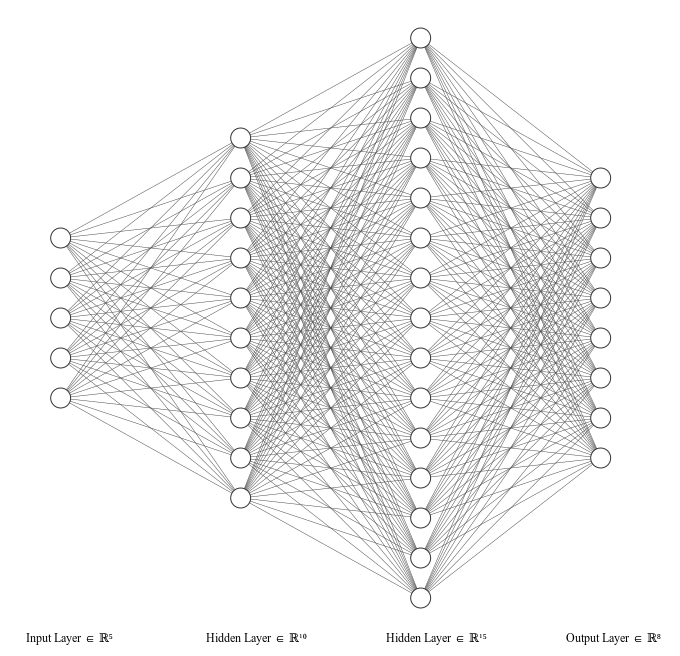
\includegraphics[width=0.6\textwidth]{img/nn.png}
    \caption{Poglądowy schemat sieci neuronowej.}
    \label{fig:neural_network}
\end{figure}
W tym badaniu ustalono optymalną architekturę sieci neuronowej na 4 warstwy:
\begin{itemize}
    \item warstwa wejściowa - 16 neuronów, po jednym na każdą cechę
    \item pierwsza warstwa ukryta - 128 neuronów
    \item druga warstwa ukryta - 256 neuronów
    \item warstwa wyjściowa - 26 neuronów, po jednym na każdą literę alfabetu angielskiego.
\end{itemize}
\subsubsection{Funkcja aktywacji}\label{subsubsec:funkcja_aktywacji}
Funkcja aktywacji jest funkcją, która przekształca sumę ważoną wejść neuronu na jego wyjście.
Gdyby nie było funkcji aktywacji, to sieć neuronowa byłaby liniowa, a wtedy nie byłaby w stanie nauczyć się złożonych zależności.
W tym badaniu użyto funkcji ReLU na warstwach ukrytych (ang. \textit{Rectified Linear Unit}) oraz softmax na wyjściowej.
\begin{equation}
    f(x) = max(0, x)
\end{equation}
\begin{figure}[H]
    \centering
    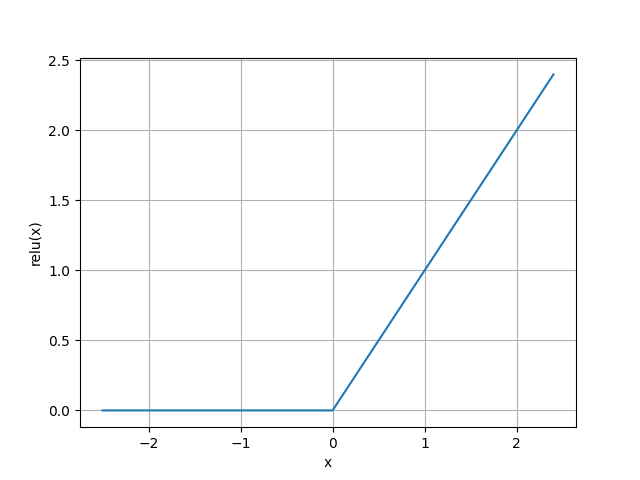
\includegraphics[width=0.6\textwidth]{img/relu.png}
    \caption{Funkcja ReLU.}
    \label{fig:relu}
\end{figure}
Funkcja softmax jest funkcją, która przekształca wektor liczb rzeczywistych na wektor liczb z przedziału [0, 1].
Suma wszystkich wartości wektora wyjściowego jest równa 1, więc można go interpretować jako rozkład prawdopodobieństwa.
W przypadku użycia jako funkcja aktywacji w warstwie wyjściowej, największa wartość wektora wyjściowego traktowana jest jako wynik klasyfikacji.
\begin{equation}
    \label{eq:softmax}
    f(x_i) = \frac{e^{x_i}}{\sum_{j=1}^{n} e^{x_j}}
\end{equation}
\subsubsection{Funkcja straty}\label{subsubsec:funkcja_straty}
Funkcja straty jest funkcją, która określa jak bardzo wynik klasyfikacji różni się od oczekiwanego.
Ze względu na to, że wyjście sieci neuronowej nie jest przedstawiona jako wektor one-hot
(wektor, w którym tylko jedna wartość jest równa 1, a reszta 0),
wykorzystano funkcję entropii krzyżowej kategorycznej (ang. \textit{sparse categorical cross-entropy}).
\begin{equation}
    f(y, \hat{y}) = -\sum_{i=1}^{n} y_i \log(\hat{y_i}),
\end{equation}
gdzie $y$ to wektor oczekiwanych wyjść, a $\hat{y}$ to wektor wyjść sieci neuronowej.
\subsubsection{Uczenie sieci}\label{subsubsec:uczenie_sieci}
Uczenie sieci neuronowej polega na aktualizacji wag połączeń między neuronami.
Najważniejszymi parametrami podczas trenowania sieci neuronowej są:
\begin{itemize}
    \item współczynnik uczenia (ang. \textit{learning rate}) - określa jak bardzo aktualizowane są wagi po każdej iteracji.
    \item funkcja optymalizująca (ang. \textit{optimizer}) - określa jak aktualizowane są wagi po każdej iteracji.
    \item funkcja straty (ang. \textit{loss function}) - określa jak bardzo wynik klasyfikacji różni się od oczekiwanego.
    \item liczba epok (ang. \textit{epochs}) - określa ile razy sieć neuronowa przejdzie przez cały zbiór danych.
\end{itemize}
W tym badaniu użyto następujących parametrów:
\begin{itemize}
    \item współczynnik uczenia - 0.001
    \item funkcja optymalizująca - Adam
    \item funkcja straty - entropia krzyżowa kategoryczna
    \item liczba epok - 40
\end{itemize}
\subsubsection{Czas trenowania}\label{subsubsec:czas_trenowania_nn}
Czas trenowania sieci neuronowej zależy od wielu czynników, takich jak:
\begin{itemize}
    \item liczba warstw
    \item liczba neuronów w warstwach
    \item liczba epok
    \item liczba danych
    \item złożoność danych
    \item parametry trenowania
    \item sprzęt
\end{itemize}
Jak wcześniej wspomniano, sieć jest relatywnie mała i prosta, dane niezbyt obszerne, ani złożone, a parametry trenowania nie są zbyt wymagające.
W związku z tym, czas trenowania sieci neuronowej nie jest długi, nawet na słabszym sprzęcie.
Do trenowania wykorzystano łatwo dostępny sprzęt, który nie jest dedykowany do uczenia maszynowego: procesor AMD Ryzen 5 5600 6-core 3.7 GHz wraz z 32 GB RAM.
Czas trenowania sieci neuronowej wyniósł około 15 sekund dla danych niezbalansowanych, 17 dla oversampled oraz około 13 dla undersampled.
\subsubsection{Dokładność i strata podczas treningu}\label{subsubsec:dokladnosc_i_strata_podczas_treningu}
Dokładność i strata podczas treningu są miarami określającymi, jak dobrze sieć neuronowa radzi sobie z klasyfikacją na zbiorze walidacyjnym po każdej iteracji trenowania.
W idealnym świecie dokładność osiąga 100\%, a strata jest bliska 0. Jednak w rzeczywistości nie jest to możliwe, bądź nie jest to opłacalne.
Ryzykujemy bowiem przeuczeniem sieci neuronowej, co oznacza, że sieć będzie zbyt dobrze radzić sobie z danymi treningowymi, ale nie będzie w stanie dobrze klasyfikować nowych danych.
W trenowaniu sieci neuronowej zależy nam na generalizowaniu, czyli na tym, żeby sieć dobrze radziła sobie z różnymi danymi, a nie tylko tymi, na których była trenowana.
\begin{figure}[H]
    \begin{subfigure}{.33\textwidth}
        \centering
        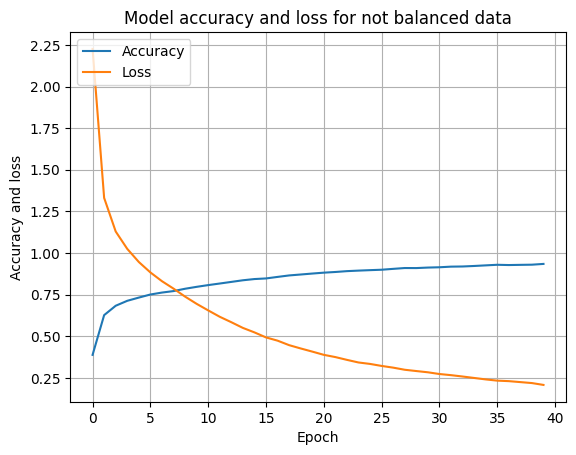
\includegraphics[width=\textwidth]{img/not_balanced_acc_loss.png}
        \caption{Niezbalansowane.}
        \label{fig:accu_loss_not_balanced}
    \end{subfigure}
    \begin{subfigure}{.33\textwidth}
        \centering
        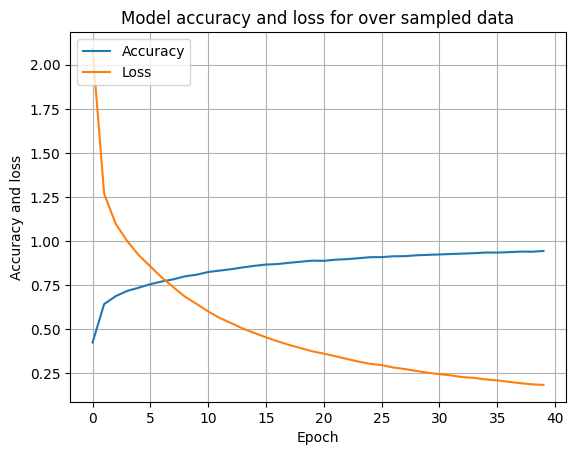
\includegraphics[width=\textwidth]{img/over_acc_loss.png}
        \caption{Oversampling.}
        \label{fig:loss}
    \end{subfigure}
    \begin{subfigure}{.33\textwidth}
        \centering
        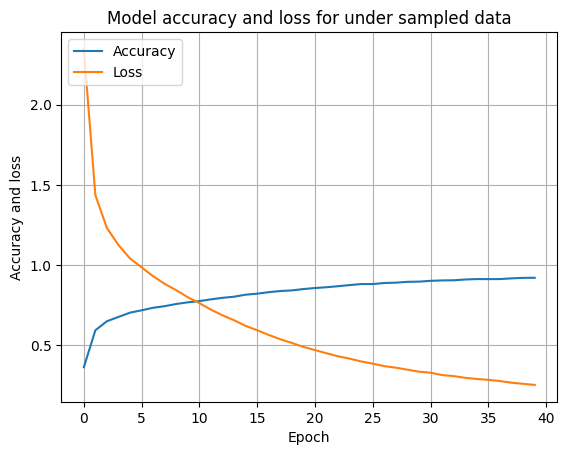
\includegraphics[width=\textwidth]{img/under_acc_loss.png}
        \caption{Undersampling.}
        \label{fig:accu_loss_under}
    \end{subfigure}
    \caption{Dokładność i strata podczas treningu względem liczby epok.}
\end{figure}
Widoczne jest duże podobieństwo między wykresami dokładności i straty dla wszystkich trzech przypadków.
Widoczne jest też poprawne zachowanie się sieci neuronowej: dokładność rośnie do 1, a strata maleje do 0.
\subsection{K najbliższych sąsiadów}\label{sec:k_najblizszych_sasiadow}
\subsubsection{Algorytm}\label{subsubsec:algorytm}
Algorytm k najbliższych sąsiadów (ang. \textit{k nearest neighbors}) jest algorytmem uczenia maszynowego, który klasyfikuje dane na podstawie ich najbliższych sąsiadów.
W przeciwieństwie do sieci neuronowej, algorytm k najbliższych sąsiadów nie uczy się na podstawie danych, tylko przechowuje je w pamięci.
Klasyfikacji dokonuje się poprzez znalezienie k najbliższych sąsiadów i wybraniu najczęściej występującej klasy.
\begin{figure}[H]
    \centering
    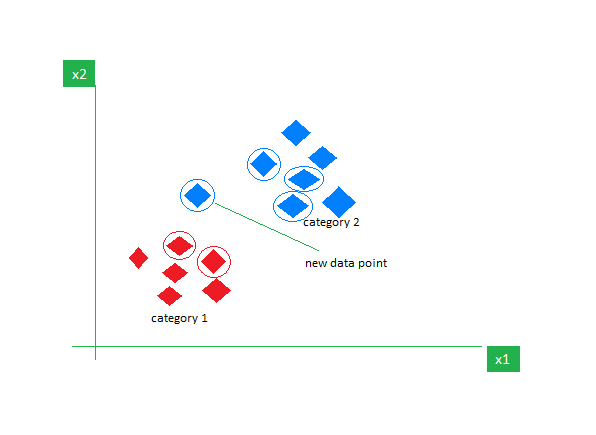
\includegraphics[width=0.8\textwidth]{img/knn.png}
    \caption{Poglądowy schemat algorytmu k najbliższych sąsiadów \cite{knn-GeeksforGeeks_2023}.}
    \label{fig:knn}
\end{figure}
\subsubsection{Parametry}\label{subsubsec:parametry}
Parametrami algorytmu k najbliższych sąsiadów są:
\begin{itemize}
    \item liczba sąsiadów (ang. \textit{n\_neighbors}) - określa ile najbliższych sąsiadów zostanie wybranych.
    \item metryka (ang. \textit{metric}) - określa jak będzie liczona odległość między danymi.
\end{itemize}
W tym badaniu użyto następujących parametrów:
\begin{itemize}
    \item liczba sąsiadów - 3
    \item metryka - euklidesowa
\end{itemize}
\subsubsection{Czas trenowania, dokładność i strata}\label{subsubsec:czas_trenowania_knn}
Tak, jak wcześniej wspomniano, algorytm k najbliższych sąsiadów tylko przechowuje w pamięci dane treningowe, a co za tym idzie, nie wymaga trenowania - czas jest równy 0 
(pomijając elementy czysto sprzętowo-techniczne jak odczytanie i załadowanie danych do pamięci).
Z tego też powodu dokładność i strata nie są miarami, które można określić dla algorytmu k najbliższych sąsiadów.

    \section{Testowanie}\label{sec:testowanie}
\subsection{Sieć neuronowa}\label{subsec:testowanie_siec_neuronowa}
Ważnym elementem każdego modelu uczenia maszynowego jest sprawdzenie, jak model radzi sobie z danymi, których nie widział podczas uczenia.
W tym celu wykorzystuje się zbiór testowy zawierający dane, które nie były użyte do trenowania modelu.
Wyniki klasyfikacji na zbiorze testowym są miarą tego, jak dobrze model radzi sobie z nowymi danymi - jak bardzo model jest w stanie generalizować swoją wiedzę.
\begin{table}[H]
    \centering
    \caption{Dokładność i F-miara dla zbioru testowego po 40 epokach}
    \resizebox{0.6\textwidth}{!}{%
        \begin{tabular}{@{}|l|l|l|l|@{}}
            \toprule
                       & Niezbalansowane & Over sampling & Under sampling \\ \midrule
            dokładność & 91\%         & 92\%       & 90\%        \\ \midrule
            F-miara    & 0,91          & 0,92        & 0,90         \\ \bottomrule
        \end{tabular}%
    }
    \label{tab:acc_f_measure_nn}
\end{table}
Powyższa tabela \ref{tab:acc_f_measure_nn} przedstawia wyniki dokładności i F-miary dla zbioru testowego. Widać wyraźnie, że wyniki są bardzo zbliżone do siebie różniąc się o maksymalnie 2 punkty procentowe.
F-miara również jest praktycznie taka sama dla wszystkich trzech zbiorów, a co najważniejsze, ich wartość oscyluje w okolicach 90\%. Świadczy to o tym, że model radzi sobie dobrze z nowymi danymi oraz
nie ma problemu z rozpoznawaniem klas mniejszościowych.
\subsection{K - NN}\label{subsec:testowanie_knn}
\begin{table}[H]
    \centering
    \caption{Dokładność i F-miara dla zbioru testowego dla k = 3}
    \resizebox{0.6\textwidth}{!}{%
        \begin{tabular}{@{}|l|l|l|l|@{}}
            \toprule
                       & Niezbalansowane & Over sampling & Under sampling \\ \midrule
            dokładność & 94,41\%         & 95,29\%       & 93,38\%        \\ \midrule
            F-miara    & 0,9443          & 0,9508        & 0,9339         \\ \bottomrule
        \end{tabular}%
    }
    \label{tab:acc_f_measure_knn}
\end{table}
W przypadku algorytmu k - NN, wyniki są jeszcze lepsze niż w przypadku sieci neuronowej. Dokładność i F-miara są wyższe o około 3 punkty procentowe. Zaznaczając przy tym zerowy czas uczenia.
Można też przedstawić wyniki klasyfikacji w postaci macierzy pomyłek. Macierz pomyłek przedstawia liczbę poprawnie i niepoprawnie zaklasyfikowanych obrazów dla każdej klasy.
\begin{figure}[H]
    \centering
    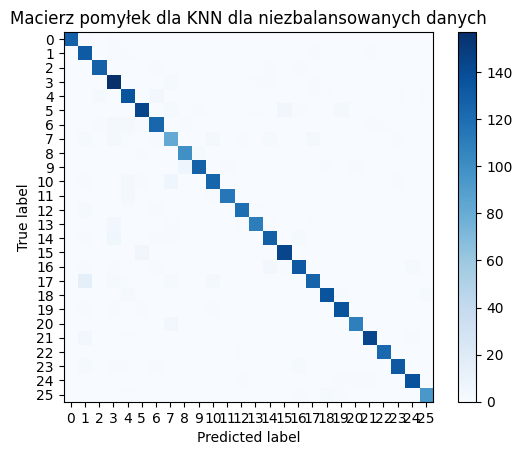
\includegraphics[width=0.5\textwidth]{img/confusion_not_balanced.png}
    \caption{Niezbalansowany zbiór testowy}
    \label{fig:confusion_matrix_knn_unbalanced}
\end{figure}
\begin{figure}[H]
    \begin{subfigure}{0.5\textwidth}
        \centering
        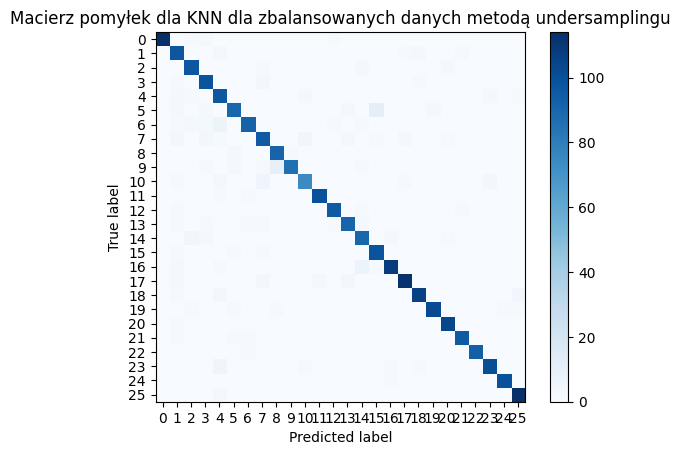
\includegraphics[width=\textwidth]{img/confusion_under.png}
        \caption{Under sampled zbiór testowy}
        \label{fig:confusion_matrix_knn_under}
    \end{subfigure}
    \begin{subfigure}{0.49\textwidth}
        \centering
        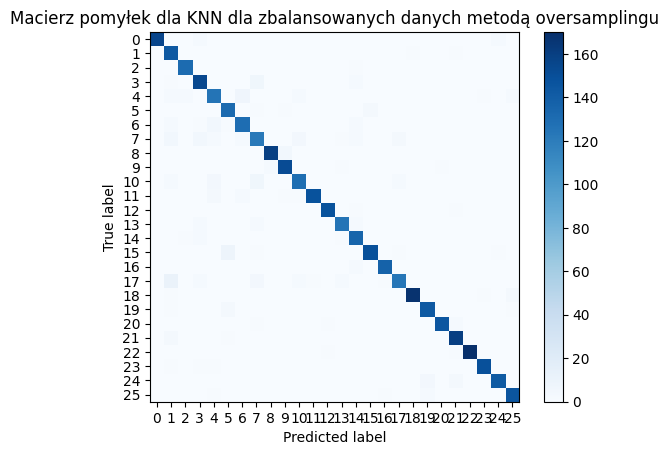
\includegraphics[width=\textwidth]{img/confusion_over.png}
        \caption{Over sampled zbiór testowy}
        \label{fig:confusion_matrix_knn_over}
    \end{subfigure}
\end{figure}
Ze względu na bardzo wysoką dokładność modelu KNN oraz bardzo niską liczbę błędów, macierz pomyłek jest bardzo podobna dla wszystkich trzech przypadków.
Widoczne są bardzo niewyraźne plamy poza przekątną głównej macierzy, co oznacza, że model dobrze radzi sobie z klasyfikacją.

    \section{Wnioski}\label{sec:wnioski}
Modele do klasyfikacji danych można trenować na różne sposoby. W tym badaniu porównano dwa modele: sieć neuronową i k - NN.
Sieć neuronowa jest modelem, który wymaga uczenia - jest więc bardziej złożona obliczeniowo, wymaga więcej czasu na trenowanie i testowanie,
natomiast sposób w jaki jest to robione jest bardziej uniwersalny, elastyczny. Sieć neuronowa może być użyta do różnych problemów, nie tylko klasyfikacji.
K - NN jest modelem, który nie wymaga uczenia - jest więc mniej złożony obliczeniowo, wymaga mniej czasu na trenowanie i testowanie,
brakuje tu jednak elastyczności. K - NN może być użyty tylko do problemów klasyfikacji. Jednak używanie wiertarki do wbicia gwoździa nie jest najlepszym pomysłem.
stąd też zależy od problemu, który model wybrać. W tym badaniu KNN dała lepsze wyniki, ale nie oznacza to, że zawsze tak będzie. W zależności od problemu,
danych, parametrów, sieć neuronowa może dać lepsze wyniki. Warto więc znać oba modele i wiedzieć, kiedy który wybrać.
    \newpage
    \bibliographystyle{unsrt}
    \bibliography{bibliography}
\end{document}
